% Quantitative figures; diagnostic development data, not official Pd/Fa.
\begin{figure*}[t]
\centering
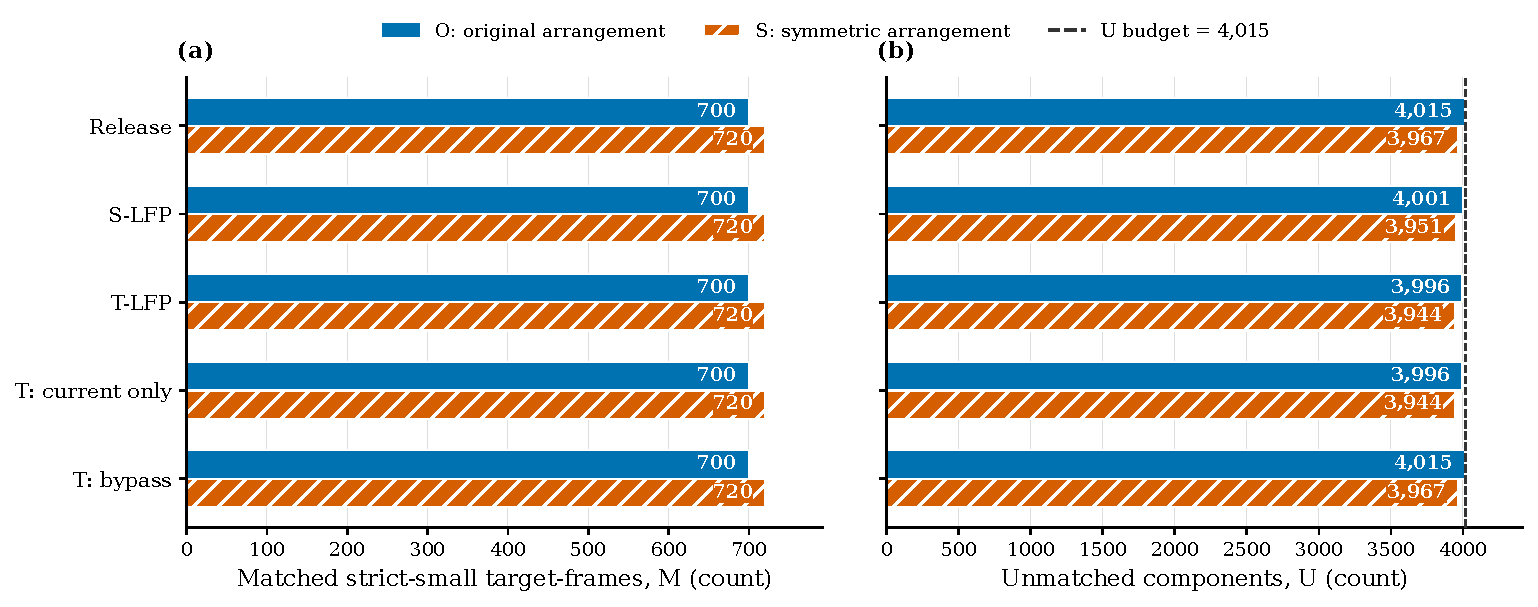
\includegraphics[width=0.95\textwidth]{visualizations/main_results.pdf}
\caption{Strict-small target-frame matches (M) and unmatched components (U) under the fixed original (O) and symmetric (S) five-window arrangements. Axes start at zero; the dashed line denotes the frozen U budget. The current-only and bypass outputs use the same T-LFP checkpoint. Results are from one seed and two development clips; these diagnostic counts are not official Pd/Fa.}
\end{figure*}

\begin{figure*}[t]
\centering
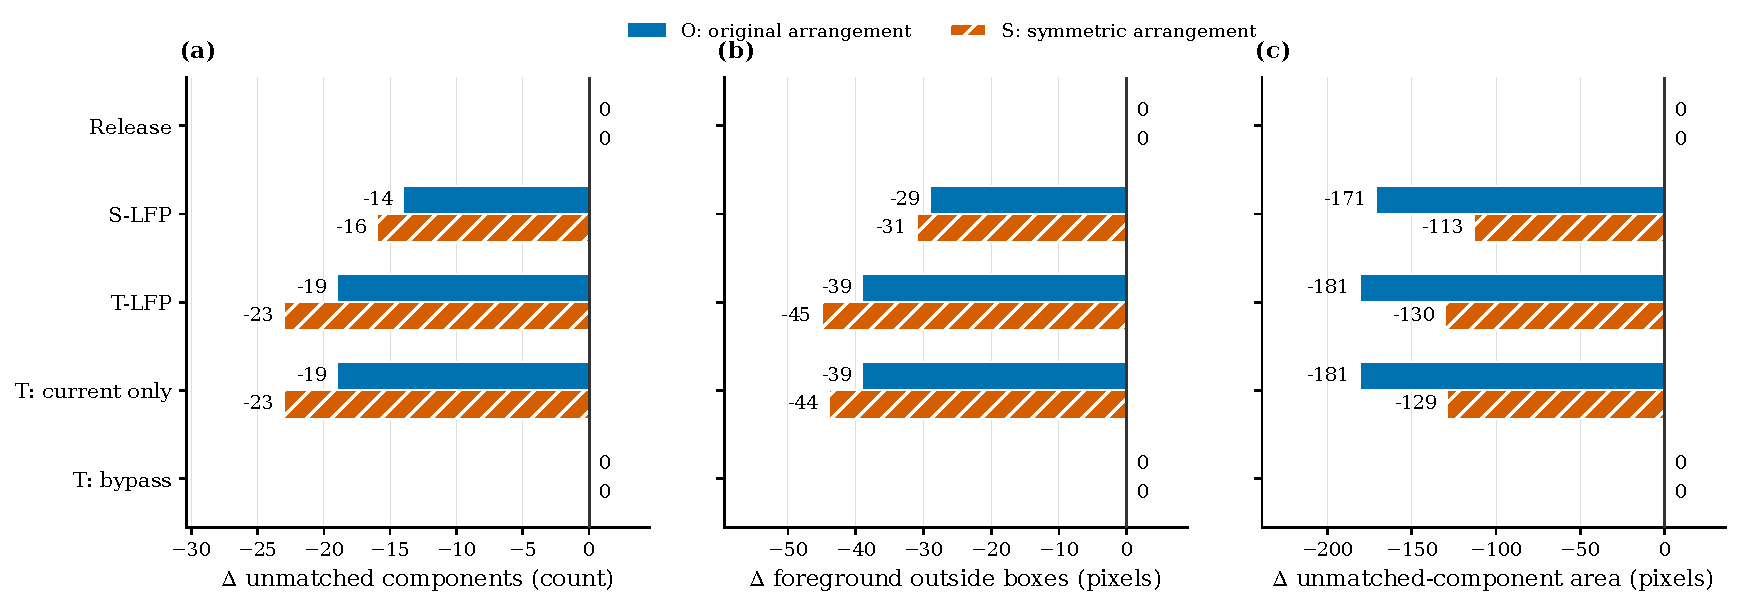
\includegraphics[width=0.95\textwidth]{visualizations/background_deltas.pdf}
\caption{Absolute changes in three recorded background costs relative to release weights under the same arrangement. Negative values denote lower costs; panels have distinct count or pixel scales. Small cost decreases do not demonstrate recovery of persistent misses.}
\end{figure*}

\begin{figure*}[t]
\centering
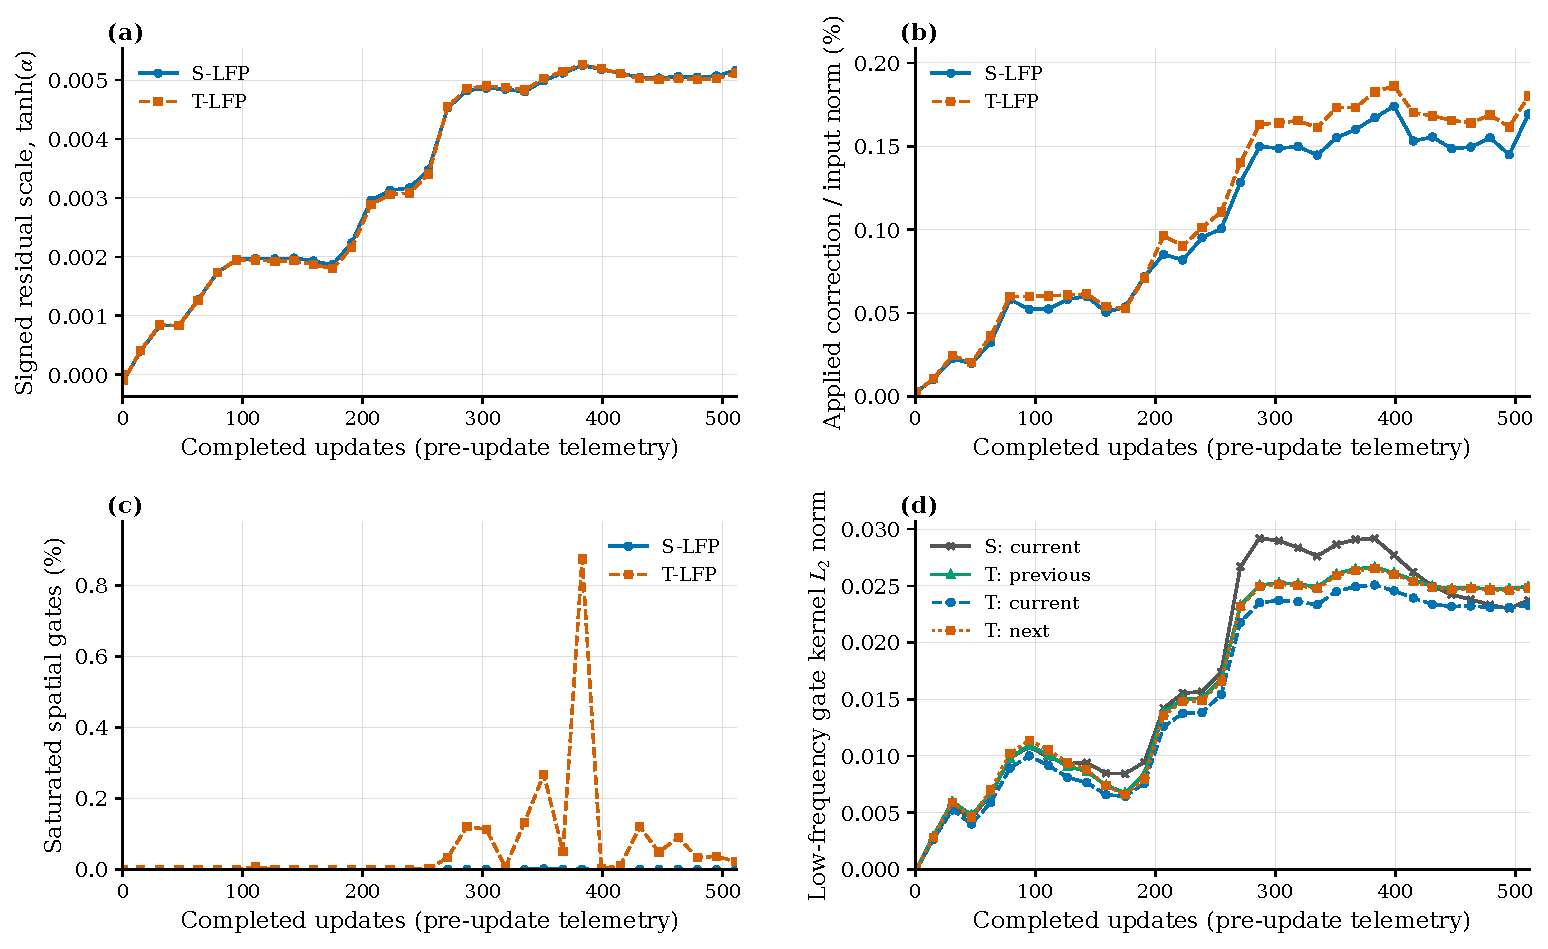
\includegraphics[width=0.95\textwidth]{visualizations/training_diagnostics.pdf}
\caption{Pre-update training telemetry: signed residual scale, applied correction-to-input norm ratio, saturated spatial-gate fraction, and low-frequency gate kernel norms. Markers are saved samples; lines connect samples without smoothing. The x coordinate is logged step minus one, so the last sample precedes the final update. These are training diagnostics, not detection performance or causal evidence of recovery.}
\end{figure*}
